\begin{frame}{implementing locks: single core}
    \begin{itemize}
    \item intuition: context switch only happens on interrupt
        \begin{itemize}
        \item timer expiration, I/O, etc. causes OS to run
        \end{itemize}
    \item solution: disable them
        \begin{itemize}
        \item reenable on unlock
        \end{itemize}
    \item<2-> x86 instructions:
        \begin{itemize}
        \item \texttt{cli} --- disable interrupts
        \item \texttt{sti} --- enable interrupts
        \end{itemize}
    \end{itemize}
\end{frame}

\begin{frame}[fragile,label=naiveEnableDisable1]{naive interrupt enable/disable (1)}
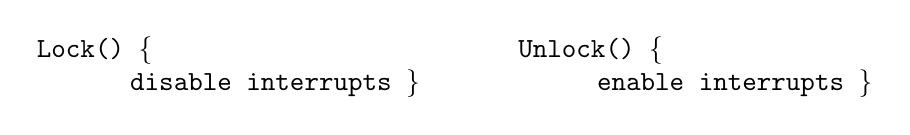
\begin{tikzpicture}
\node[align=left,font=\tt] (lock code) {
Lock() \{ \\
\hspace{1cm} \myemph{disable interrupts}
\} 
};
\node[anchor=north west,align=left,font=\tt] (unlock code) at ([xshift=1cm]lock code.north east) {
Unlock() \{ \\
\hspace{1cm}\myemph{enable interrupts}
\}
};
\end{tikzpicture}
\begin{itemize}
\item<2-> problem: user can \myemph{hang the system}:
\begin{lstlisting}[
    language=C++,
    style=small,
    moredelim={**[is][\btHL<1-|handout:1->]{@1}{1@}},
]    
            Lock(some_lock);
            while (true) {}
\end{lstlisting}
\item<3-> problem: can't do I/O within lock
\begin{lstlisting}[
    language=C++,
    style=small,
    moredelim={**[is][\btHL<1-|handout:1->]{@1}{1@}},
]    
            Lock(some_lock);
            read from disk
                /* waits forever for (disabled) interrupt
                   from disk IO finishing */
\end{lstlisting}
\end{itemize}
\end{frame}


\begin{frame}[fragile,label=naiveEnableDisable2]{naive interrupt enable/disable (2)}
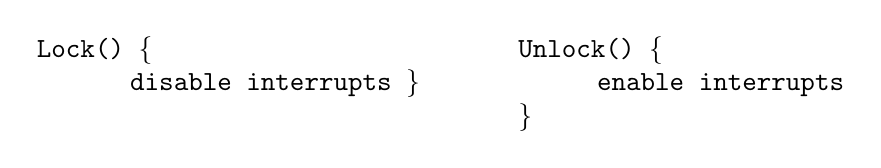
\begin{tikzpicture}
\node[align=left,font=\tt] (lock code) {
Lock() \{ \\
\hspace{1cm} \myemph{disable interrupts}
\} 
};
\node[anchor=north west,align=left,font=\tt] (unlock code) at ([xshift=1cm]lock code.north east) {
Unlock() \{ \\
\hspace{1cm}\myemph{enable interrupts} \\
\}
};
\end{tikzpicture}
\begin{itemize}
\item<4-> problem: nested locks
\begin{lstlisting}[
    language=C++,
    style=small,
    moredelim={**[is][\color{red}\bfseries]{@1}{1@}},
]    
        Lock(milk_lock);
        if (no milk) {
            Lock(store_lock);
            buy milk
            Unlock(store_lock);
            /* interrupts enabled here?? */
        }
        Unlock(milk_lock);
\end{lstlisting}
\end{itemize}
\end{frame}

